\documentclass[11pt,a4paper]{report}
\usepackage[utf8]{inputenc}
\usepackage{amsmath}
\usepackage{lscape}
\usepackage{amsfonts}
\usepackage{amssymb}
\usepackage{graphicx}
\usepackage{pdfpages}
\begin{document}
\section*{Contínua}
\begin{center}
	\hspace*{-3.5cm}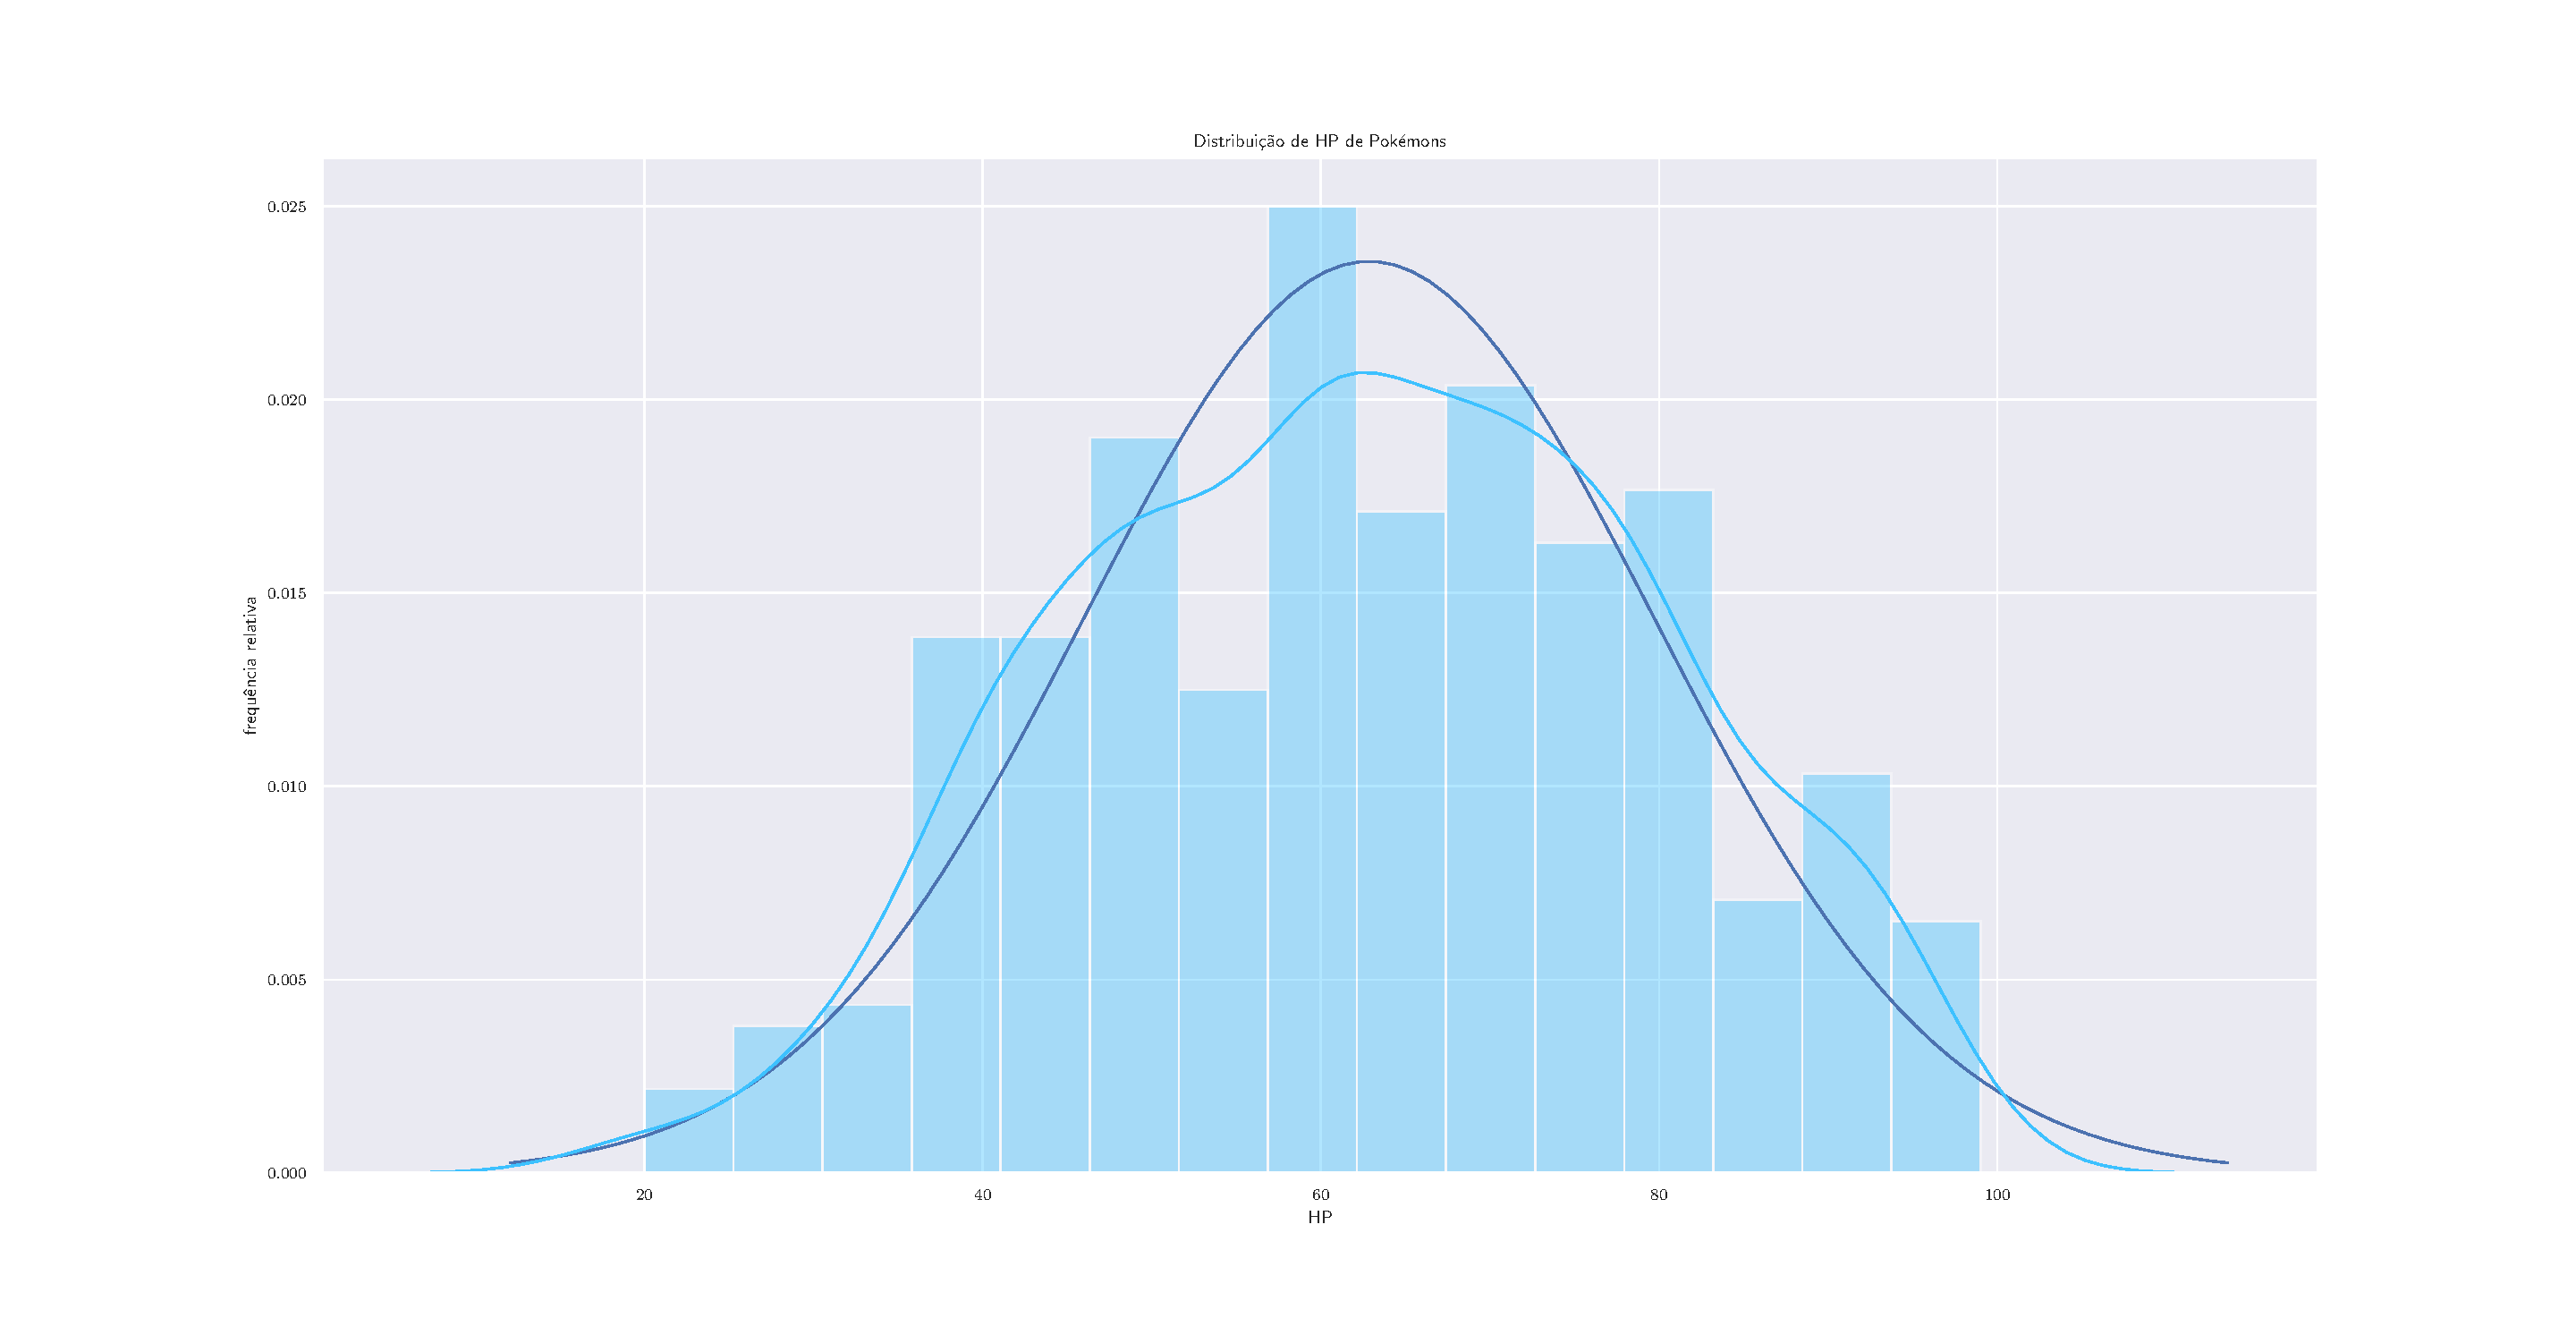
\includegraphics[clip, trim=0cm 0cm 0.0cm 0cm, width=1.7\linewidth]{continua.pdf}

\end{center}
V.A.: Número de Hit Points de um Pokémon. \\
Distribuição aproximada: Normal.\\
Se subentende que por motivos de balanceamento, os criadores do jogo decidam que poucos personagens possuam muito ou pouco pontos de vida. ({\it Hit Points})\\
No gráfico, a distribuição calculada é dada pela curva azul-forte.\\
A distribuição aproximada calculada pelo sistema é dada pela curva azul fraco.\\

\section*{Discreta}
\begin{center}
	\hspace*{-3.5cm}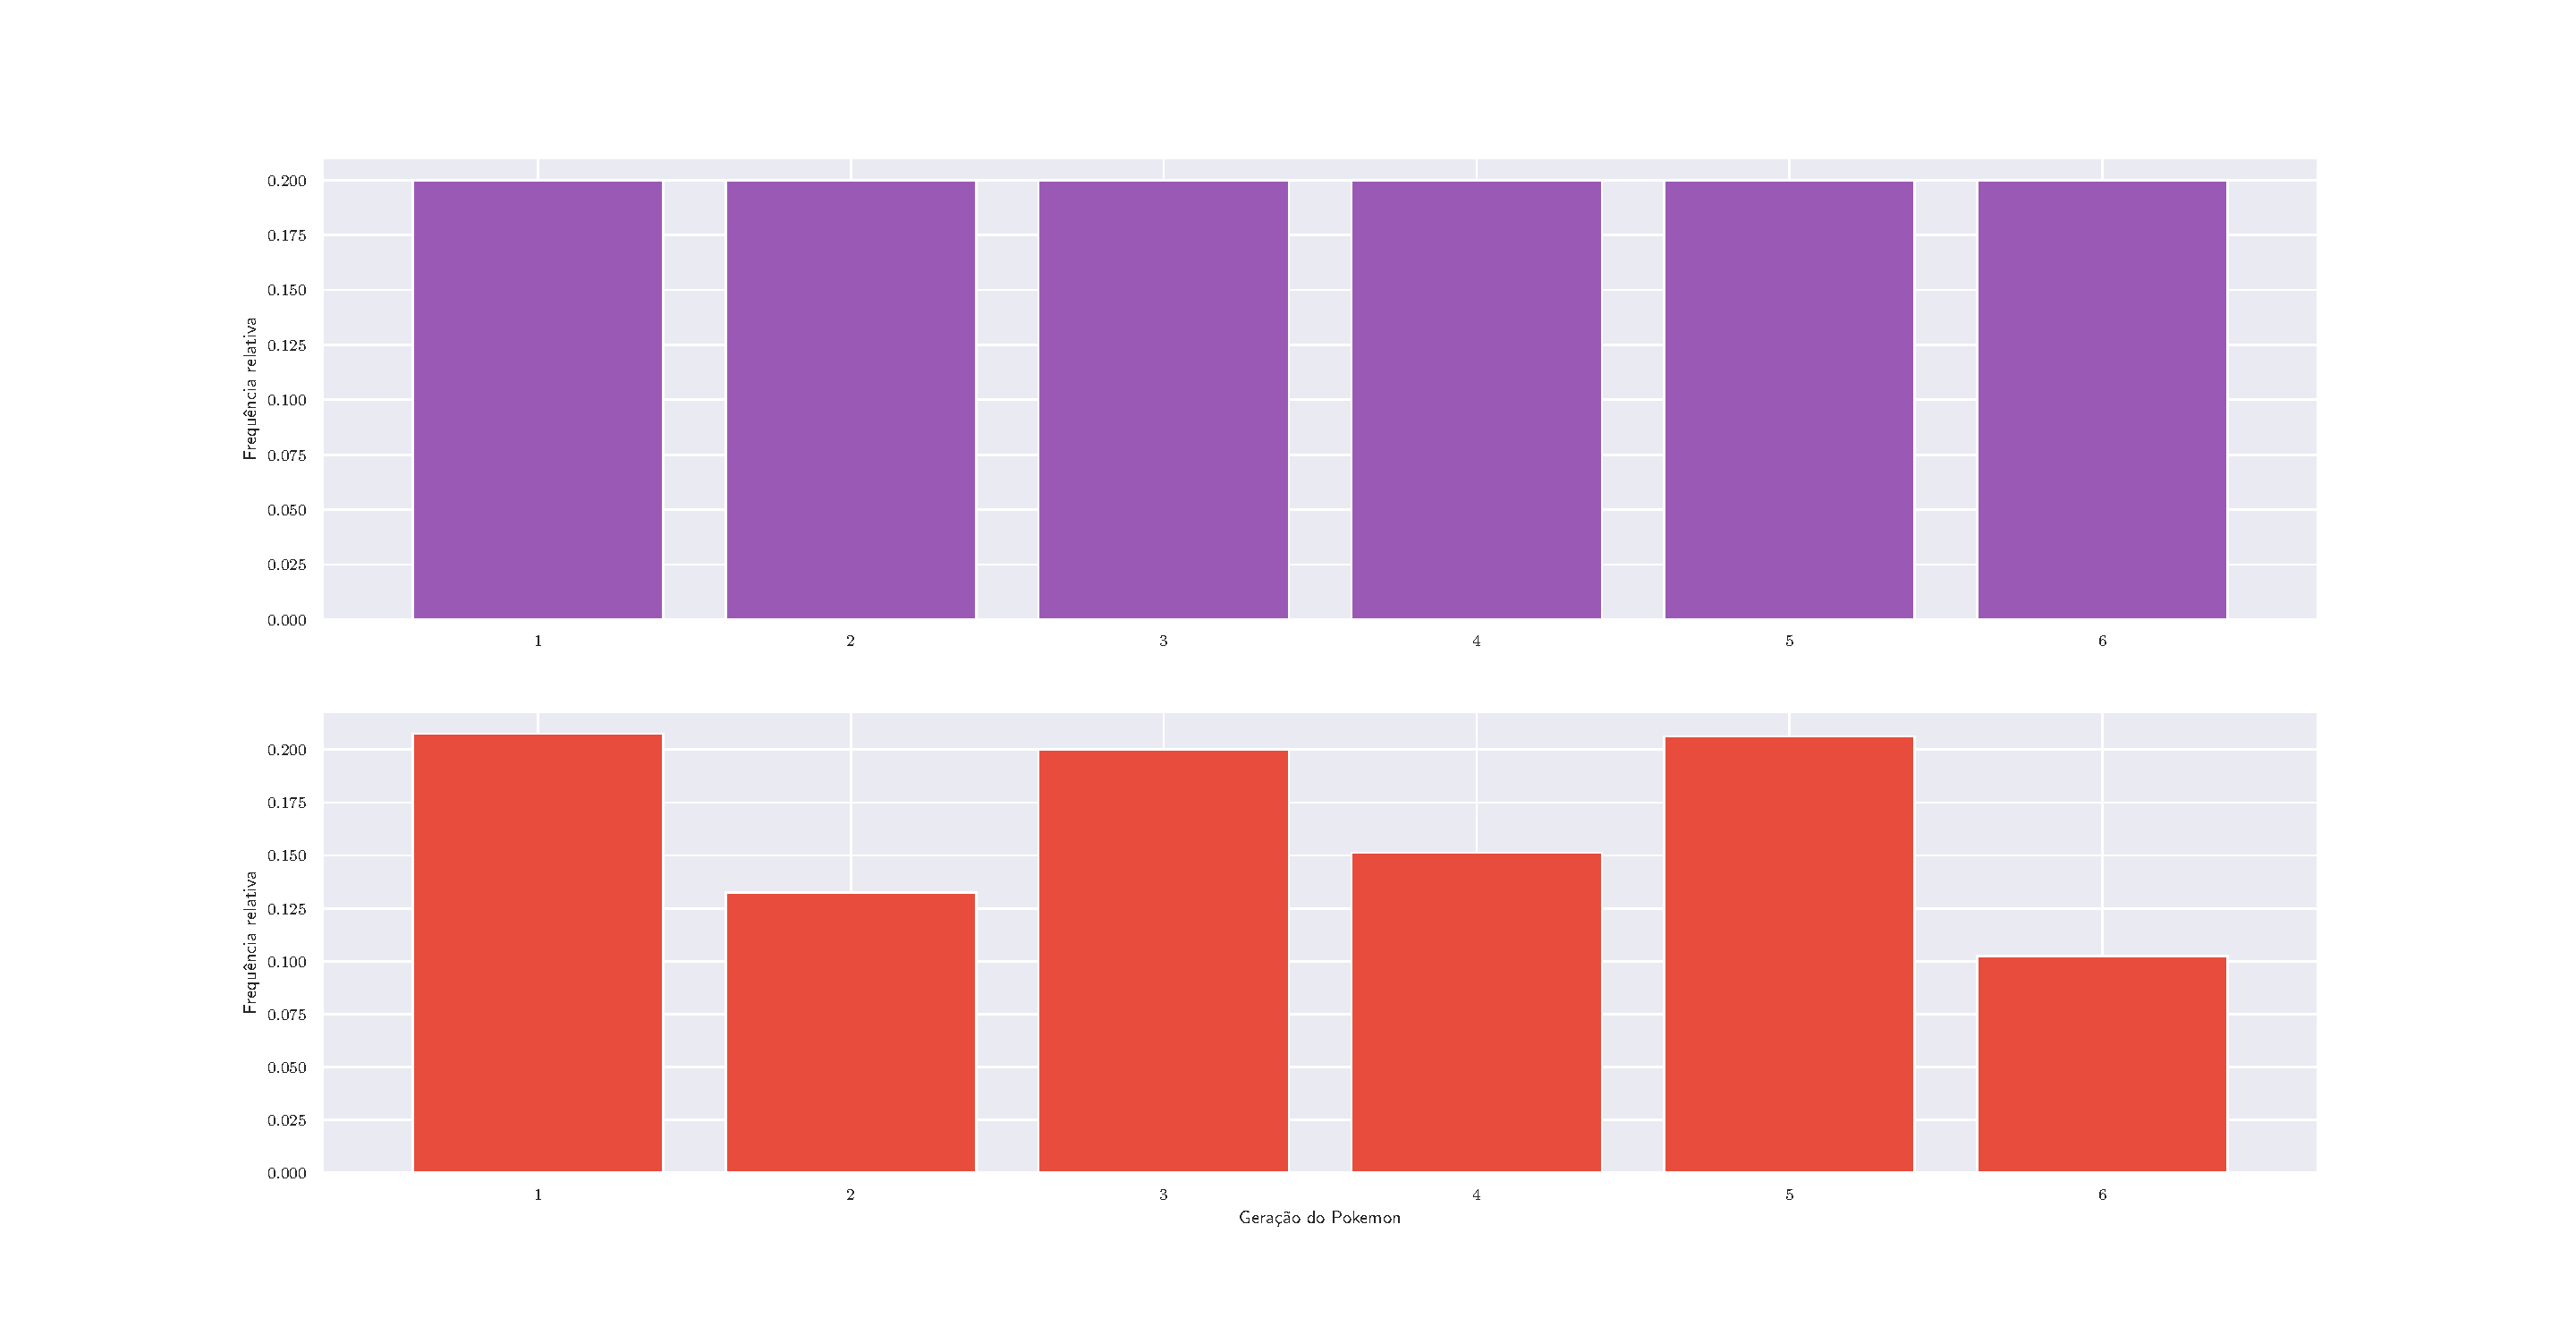
\includegraphics[clip, trim=0cm 0cm 0.0cm 0cm, width=1.7\linewidth]{discreta.pdf}
	
\end{center}
V.A.: Número da Geração de um Pokemón.\\
Distribuição aproximada: Uniforme Discreta.\\
Se subentende que os criadores do jogo lançam a mesma quantidade de personagens por geração.

\end{document}